% Graphic for TeX using PGF
% Title: /home/tomgli/workspace/github.com/bachopp/thesis/files/chapters/design/graphics/advancedfluxaddstudent.dia
% Creator: Dia v0.97.3
% CreationDate: Sat May  7 17:20:12 2016
% For: tomgli
% \usepackage{tikz}
% The following commands are not supported in PSTricks at present
% We define them conditionally, so when they are implemented,
% this pgf file will use them.
\ifx\du\undefined
  \newlength{\du}
\fi
\setlength{\du}{15\unitlength}
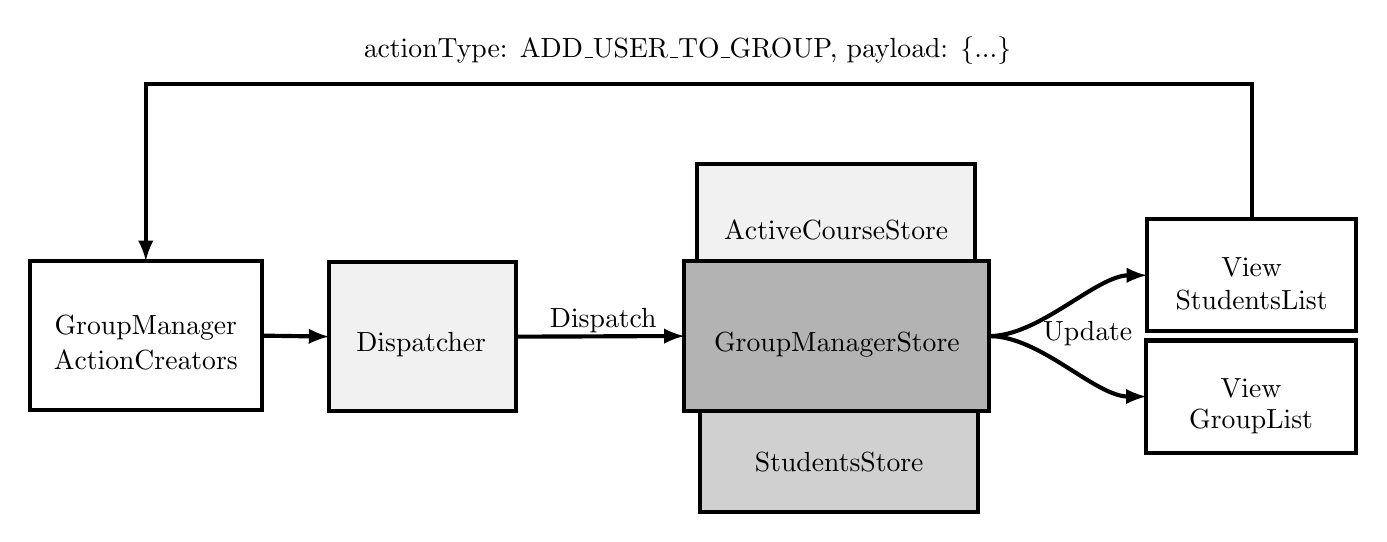
\begin{tikzpicture}
\pgftransformxscale{1.000000}
\pgftransformyscale{-1.000000}
\definecolor{dialinecolor}{rgb}{0.000000, 0.000000, 0.000000}
\pgfsetstrokecolor{dialinecolor}
\definecolor{dialinecolor}{rgb}{1.000000, 1.000000, 1.000000}
\pgfsetfillcolor{dialinecolor}
\definecolor{dialinecolor}{rgb}{1.000000, 1.000000, 1.000000}
\pgfsetfillcolor{dialinecolor}
\fill (3.451510\du,5.177804\du)--(3.451510\du,8.779196\du)--(9.041885\du,8.779196\du)--(9.041885\du,5.177804\du)--cycle;
\pgfsetlinewidth{0.100000\du}
\pgfsetdash{}{0pt}
\pgfsetdash{}{0pt}
\pgfsetmiterjoin
\definecolor{dialinecolor}{rgb}{0.000000, 0.000000, 0.000000}
\pgfsetstrokecolor{dialinecolor}
\draw (3.451510\du,5.177804\du)--(3.451510\du,8.779196\du)--(9.041885\du,8.779196\du)--(9.041885\du,5.177804\du)--cycle;
% setfont left to latex
\definecolor{dialinecolor}{rgb}{0.000000, 0.000000, 0.000000}
\pgfsetstrokecolor{dialinecolor}
\node at (6.246697\du,6.778500\du){GroupManager};
% setfont left to latex
\definecolor{dialinecolor}{rgb}{0.000000, 0.000000, 0.000000}
\pgfsetstrokecolor{dialinecolor}
\node at (6.246697\du,7.578500\du){ActionCreators};
\definecolor{dialinecolor}{rgb}{0.945098, 0.945098, 0.945098}
\pgfsetfillcolor{dialinecolor}
\fill (10.661166\du,5.201500\du)--(10.661166\du,8.802892\du)--(15.166040\du,8.802892\du)--(15.166040\du,5.201500\du)--cycle;
\pgfsetlinewidth{0.100000\du}
\pgfsetdash{}{0pt}
\pgfsetdash{}{0pt}
\pgfsetmiterjoin
\definecolor{dialinecolor}{rgb}{0.000000, 0.000000, 0.000000}
\pgfsetstrokecolor{dialinecolor}
\draw (10.661166\du,5.201500\du)--(10.661166\du,8.802892\du)--(15.166040\du,8.802892\du)--(15.166040\du,5.201500\du)--cycle;
% setfont left to latex
\definecolor{dialinecolor}{rgb}{0.000000, 0.000000, 0.000000}
\pgfsetstrokecolor{dialinecolor}
\node[anchor=east] at (14.716040\du,7.202196\du){Dispatcher};
\pgfsetlinewidth{0.100000\du}
\pgfsetdash{}{0pt}
\pgfsetdash{}{0pt}
\pgfsetbuttcap
{
\definecolor{dialinecolor}{rgb}{0.000000, 0.000000, 0.000000}
\pgfsetfillcolor{dialinecolor}
% was here!!!
\pgfsetarrowsend{latex}
\definecolor{dialinecolor}{rgb}{0.000000, 0.000000, 0.000000}
\pgfsetstrokecolor{dialinecolor}
\draw (9.041885\du,6.978500\du)--(10.661166\du,7.002196\du);
}
\pgfsetlinewidth{0.100000\du}
\pgfsetdash{}{0pt}
\pgfsetdash{}{0pt}
\pgfsetmiterjoin
\pgfsetbuttcap
{
\definecolor{dialinecolor}{rgb}{0.000000, 0.000000, 0.000000}
\pgfsetfillcolor{dialinecolor}
% was here!!!
\pgfsetarrowsend{latex}
{\pgfsetcornersarced{\pgfpoint{0.000000\du}{0.000000\du}}\definecolor{dialinecolor}{rgb}{0.000000, 0.000000, 0.000000}
\pgfsetstrokecolor{dialinecolor}
\draw (32.886264\du,4.175125\du)--(32.886264\du,0.920171\du)--(6.246697\du,0.920171\du)--(6.246697\du,5.177804\du);
}}
% setfont left to latex
\definecolor{dialinecolor}{rgb}{0.000000, 0.000000, 0.000000}
\pgfsetstrokecolor{dialinecolor}
\node at (19.297331\du,0.115327\du){actionType: ADD\_USER\_TO\_GROUP, payload: \{...\}};
% setfont left to latex
\definecolor{dialinecolor}{rgb}{0.000000, 0.000000, 0.000000}
\pgfsetstrokecolor{dialinecolor}
\node at (28.935909\du,6.939440\du){Update};
% setfont left to latex
\definecolor{dialinecolor}{rgb}{0.000000, 0.000000, 0.000000}
\pgfsetstrokecolor{dialinecolor}
\node at (17.266210\du,6.615953\du){Dispatch};
\definecolor{dialinecolor}{rgb}{1.000000, 1.000000, 1.000000}
\pgfsetfillcolor{dialinecolor}
\fill (30.348442\du,7.095992\du)--(30.348442\du,9.795992\du)--(35.396324\du,9.795992\du)--(35.396324\du,7.095992\du)--cycle;
\pgfsetlinewidth{0.100000\du}
\pgfsetdash{}{0pt}
\pgfsetdash{}{0pt}
\pgfsetmiterjoin
\definecolor{dialinecolor}{rgb}{0.000000, 0.000000, 0.000000}
\pgfsetstrokecolor{dialinecolor}
\draw (30.348442\du,7.095992\du)--(30.348442\du,9.795992\du)--(35.396324\du,9.795992\du)--(35.396324\du,7.095992\du)--cycle;
% setfont left to latex
\definecolor{dialinecolor}{rgb}{0.000000, 0.000000, 0.000000}
\pgfsetstrokecolor{dialinecolor}
\node at (32.872383\du,8.245992\du){View};
% setfont left to latex
\definecolor{dialinecolor}{rgb}{0.000000, 0.000000, 0.000000}
\pgfsetstrokecolor{dialinecolor}
\node at (32.872383\du,9.045992\du){GroupList};
\pgfsetlinewidth{0.100000\du}
\pgfsetdash{}{0pt}
\pgfsetdash{}{0pt}
\pgfsetmiterjoin
\pgfsetbuttcap
{
\definecolor{dialinecolor}{rgb}{0.000000, 0.000000, 0.000000}
\pgfsetfillcolor{dialinecolor}
% was here!!!
\pgfsetarrowsend{latex}
\definecolor{dialinecolor}{rgb}{0.000000, 0.000000, 0.000000}
\pgfsetstrokecolor{dialinecolor}
\pgfpathmoveto{\pgfpoint{26.567568\du}{6.989368\du}}
\pgfpathcurveto{\pgfpoint{27.781372\du}{6.989368\du}}{\pgfpoint{29.148519\du}{5.525125\du}}{\pgfpoint{30.362323\du}{5.525125\du}}
\pgfusepath{stroke}
}
\pgfsetlinewidth{0.100000\du}
\pgfsetdash{}{0pt}
\pgfsetdash{}{0pt}
\pgfsetmiterjoin
\pgfsetbuttcap
{
\definecolor{dialinecolor}{rgb}{0.000000, 0.000000, 0.000000}
\pgfsetfillcolor{dialinecolor}
% was here!!!
\pgfsetarrowsend{latex}
\definecolor{dialinecolor}{rgb}{0.000000, 0.000000, 0.000000}
\pgfsetstrokecolor{dialinecolor}
\pgfpathmoveto{\pgfpoint{26.567568\du}{6.989368\du}}
\pgfpathcurveto{\pgfpoint{27.797615\du}{6.989368\du}}{\pgfpoint{29.118395\du}{8.445992\du}}{\pgfpoint{30.348442\du}{8.445992\du}}
\pgfusepath{stroke}
}
\definecolor{dialinecolor}{rgb}{0.815686, 0.815686, 0.815686}
\pgfsetfillcolor{dialinecolor}
\fill (19.605766\du,8.416369\du)--(19.605766\du,11.230156\du)--(26.299389\du,11.230156\du)--(26.299389\du,8.416369\du)--cycle;
\pgfsetlinewidth{0.100000\du}
\pgfsetdash{}{0pt}
\pgfsetdash{}{0pt}
\pgfsetmiterjoin
\definecolor{dialinecolor}{rgb}{0.000000, 0.000000, 0.000000}
\pgfsetstrokecolor{dialinecolor}
\draw (19.605766\du,8.416369\du)--(19.605766\du,11.230156\du)--(26.299389\du,11.230156\du)--(26.299389\du,8.416369\du)--cycle;
% setfont left to latex
\definecolor{dialinecolor}{rgb}{0.000000, 0.000000, 0.000000}
\pgfsetstrokecolor{dialinecolor}
\node at (22.952577\du,10.023262\du){StudentsStore};
\pgfsetlinewidth{0.100000\du}
\pgfsetdash{}{0pt}
\pgfsetdash{}{0pt}
\pgfsetmiterjoin
\pgfsetbuttcap
{
\definecolor{dialinecolor}{rgb}{0.000000, 0.000000, 0.000000}
\pgfsetfillcolor{dialinecolor}
% was here!!!
\pgfsetarrowsend{latex}
\definecolor{dialinecolor}{rgb}{0.000000, 0.000000, 0.000000}
\pgfsetstrokecolor{dialinecolor}
\pgfpathmoveto{\pgfpoint{15.166040\du}{7.002196\du}}
\pgfpathcurveto{\pgfpoint{16.234840\du}{7.002196\du}}{\pgfpoint{18.151423\du}{6.989368\du}}{\pgfpoint{19.220223\du}{6.989368\du}}
\pgfusepath{stroke}
}
\definecolor{dialinecolor}{rgb}{0.945098, 0.945098, 0.945098}
\pgfsetfillcolor{dialinecolor}
\fill (19.528657\du,2.834903\du)--(19.528657\du,5.648689\du)--(26.230987\du,5.648689\du)--(26.230987\du,2.834903\du)--cycle;
\pgfsetlinewidth{0.100000\du}
\pgfsetdash{}{0pt}
\pgfsetdash{}{0pt}
\pgfsetmiterjoin
\definecolor{dialinecolor}{rgb}{0.000000, 0.000000, 0.000000}
\pgfsetstrokecolor{dialinecolor}
\draw (19.528657\du,2.834903\du)--(19.528657\du,5.648689\du)--(26.230987\du,5.648689\du)--(26.230987\du,2.834903\du)--cycle;
% setfont left to latex
\definecolor{dialinecolor}{rgb}{0.000000, 0.000000, 0.000000}
\pgfsetstrokecolor{dialinecolor}
\node at (22.879822\du,4.441796\du){ActiveCourseStore};
\definecolor{dialinecolor}{rgb}{0.701961, 0.701961, 0.701961}
\pgfsetfillcolor{dialinecolor}
\fill (19.220223\du,5.188672\du)--(19.220223\du,8.790064\du)--(26.567568\du,8.790064\du)--(26.567568\du,5.188672\du)--cycle;
\pgfsetlinewidth{0.100000\du}
\pgfsetdash{}{0pt}
\pgfsetdash{}{0pt}
\pgfsetmiterjoin
\definecolor{dialinecolor}{rgb}{0.000000, 0.000000, 0.000000}
\pgfsetstrokecolor{dialinecolor}
\draw (19.220223\du,5.188672\du)--(19.220223\du,8.790064\du)--(26.567568\du,8.790064\du)--(26.567568\du,5.188672\du)--cycle;
% setfont left to latex
\definecolor{dialinecolor}{rgb}{0.000000, 0.000000, 0.000000}
\pgfsetstrokecolor{dialinecolor}
\node at (22.893895\du,7.189368\du){GroupManagerStore};
\definecolor{dialinecolor}{rgb}{1.000000, 1.000000, 1.000000}
\pgfsetfillcolor{dialinecolor}
\fill (30.362323\du,4.175125\du)--(30.362323\du,6.875125\du)--(35.410205\du,6.875125\du)--(35.410205\du,4.175125\du)--cycle;
\pgfsetlinewidth{0.100000\du}
\pgfsetdash{}{0pt}
\pgfsetdash{}{0pt}
\pgfsetmiterjoin
\definecolor{dialinecolor}{rgb}{0.000000, 0.000000, 0.000000}
\pgfsetstrokecolor{dialinecolor}
\draw (30.362323\du,4.175125\du)--(30.362323\du,6.875125\du)--(35.410205\du,6.875125\du)--(35.410205\du,4.175125\du)--cycle;
% setfont left to latex
\definecolor{dialinecolor}{rgb}{0.000000, 0.000000, 0.000000}
\pgfsetstrokecolor{dialinecolor}
\node at (32.886264\du,5.325125\du){View};
% setfont left to latex
\definecolor{dialinecolor}{rgb}{0.000000, 0.000000, 0.000000}
\pgfsetstrokecolor{dialinecolor}
\node at (32.886264\du,6.125125\du){StudentsList};
\end{tikzpicture}
